\documentclass[10pt,tikz,border=2mm]{standalone}
\usepackage{times}

\usepackage{tikz}
\usetikzlibrary{matrix}

\colorlet{helpful}{lime!70}
\colorlet{harmful}{red!30}
\colorlet{internal}{yellow!20}
\colorlet{external}{cyan!30}
\colorlet{S}{helpful!50!internal}
\colorlet{W}{harmful!50!internal}
\colorlet{O}{helpful!50!external}
\colorlet{T}{harmful!50!external}

\newcommand{\texta}{Helpful\\ \tiny (to achieve the objective)\par}
\newcommand{\textb}{Harmful\\ \tiny (to achieve the objective)\par}
\newcommand{\textcn}{Internal origin\\ \tiny (product\slash company attributes)\par}
\newcommand{\textdn}{External origin\\ \tiny (environment\slash market attributes)\par}

\newcommand{\back}[1]{\fontsize{60}{70}\selectfont #1}

\begin{document}
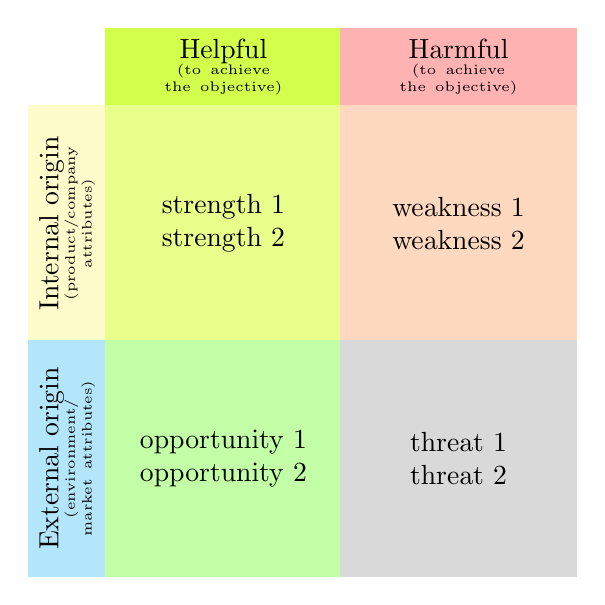
\begin{tikzpicture}[
    any/.style={minimum width=3cm,minimum height=3cm,%
                 text width=2.5cm,align=center,outer sep=0pt},
    header/.style={any,minimum height=1cm,fill=black!10},
    leftcol/.style={header,rotate=90},
    mycolor/.style={fill=#1, text=#1!60!black}
]

\matrix (SWOT) [matrix of nodes,nodes={any,anchor=center},%
                column sep=-\pgflinewidth,%
                row sep=-\pgflinewidth,%
                row 1/.style={nodes=header},%
                column 1/.style={nodes=leftcol},
                inner sep=0pt]
{
          &|[fill=helpful]| {\texta} & |[fill=harmful]| {\textb} \\
|[fill=internal]| {\textcn} & |[mycolor=S]| \back{} & |[mycolor=W]| \back{} \\
|[fill=external]| {\textdn} & |[mycolor=O]| \back{} & |[mycolor=T]| \back{} \\
};

\node[any, anchor=center] at (SWOT-2-2) {strength 1\\ strength 2};
\node[any, anchor=center] at (SWOT-2-3) {weakness 1\\ weakness 2};
\node[any, anchor=center] at (SWOT-3-2) {opportunity 1\\ opportunity 2};
\node[any, anchor=center] at (SWOT-3-3) {threat 1\\ threat 2};

\end{tikzpicture}
\end{document}